\documentclass[11pt,a4paper]{article}
\usepackage[T1]{fontenc}
\usepackage[utf8]{inputenc}
\usepackage{lmodern}
\usepackage[english]{babel}
\usepackage[a4paper,top=24mm,bottom=24mm,left=24mm,right=24mm,headheight=14pt]{geometry}
\usepackage[protrusion=true,expansion=false]{microtype}
\usepackage{parskip}
\emergencystretch=3em
\widowpenalty=10000
\clubpenalty=10000
\usepackage{amsmath,amssymb}
\usepackage{booktabs}
\usepackage{graphicx}
\usepackage{enumitem}
\usepackage[dvipsnames]{xcolor}
\usepackage{fancyhdr}
\pagestyle{fancy}
\fancyhf{}
\fancyhead[L]{\small Zoe: A Native GEM for Living Geometry and Inspectable Futures}
\fancyhead[R]{\small\thepage}
\renewcommand{\headrulewidth}{0.4pt}
\renewcommand{\footrulewidth}{0pt}
\usepackage[colorlinks=true,linkcolor=blue!60!black,urlcolor=blue!60!black,citecolor=blue!60!black,pdftitle={Zoe: A Native GEM for Living Geometry and Inspectable Futures},pdfauthor={Nicholas Michael Kloster and Zoe (AI assistant)}]{hyperref}
\usepackage{listings}
\usepackage{embedfile}
\embedfilesetup{stringmethod=escape}
\lstset{basicstyle=\ttfamily\scriptsize,breaklines=true,breakatwhitespace=false,columns=fullflexible,keepspaces=true,showstringspaces=false}

\title{\textbf{Zoe: A Native GEM for Living Geometry and Inspectable Futures}\\[5pt]
\large A Complete Proof of Concept and Verification Report}
\author{Nicholas Michael Kloster \and Zoe (AI assistant)}
\date{November 2026}

\begin{document}
\maketitle
\thispagestyle{fancy}

\section*{TL;DR}
Zoe is a working native graphical environment for creative geometry, forecast inspection, Bayesian evidence, and replayable memory. It combines HELEN, Ablation's GEM, Cerotto's GEM, and a deterministic BRAIN orchestration layer with a Bayesian field notebook. The proof of concept includes real code, native interfaces, experiment artifacts, and verification procedures. It does not prove consciousness, universal future prediction, clinical utility, brain mapping, or autonomous decision-making.

\textbf{What was built.} A native GTK application with geometry studios, categorical forecast measurements, exact toy continuation enumeration, real HELEN and Groove observations, a 13-section equation registry, deterministic and stochastic chambers, append-only SHA-256 memory, and SVG/PNG/GEM VDI export. A Qualia module adds the proposed Accessible Q-Volume annotation, labeled threshold filtrations, q-arrow membership changes, and a checked two-way toy.

\textbf{What was verified.} Twenty-five Zoe tests and 20 broader GEM tests passed under native X11. Seventeen research conformance checks passed. Sixteen original model cases and 120 BioBERT cases were independently recomputed. Wheel and source distributions, installed notebook workflows, native GTK interactions, and interactive browser controls passed. Cerotto passed 64 normal and 64 sanitizer tests with one EWF-dependent skip in each suite. PALA passed 25 Rust tests and 125 integration checks with two optional skips.

\textbf{What remains limited.} Accessible volume measures forecast breadth, not correctness or human surprise. Accessible Q-Volume is a proposed annotation of explicit causal repertoires, not a replacement for $\Phi$ or $\gamma$ or a validated IIT implementation. HOP is a rejected baseline. Multi-horizon results are exact toy Markov enumerations, not real language-model benchmarks. Nightingale is aggregate-only in the saved evidence. Posteriors follow user-supplied likelihoods. The memory chain supplies tamper evidence, not authentication. Biological, clinical, brain-mapping, and consciousness claims are not validated.

\begin{abstract}
Zoe is a native graphical environment for exploring how forecasts, measurements, beliefs, and actions differ. It unifies HELEN's lightweight geometry and stored predictions, Ablation's Spatial IR and VDI evidence environment, Cerotto's forensic workbench, and BRAIN's deterministic observation and recommendation layer. Its Bayesian field notebook adds questions, competing claims, explicit likelihoods, dependent-evidence barriers, deterministic and stochastic chambers, and append-only memory. This paper documents the complete proof of concept: the accessible-volume equation and its development, temporal and geometric formulations, native GEM versions, Bayesian memory, native interfaces, and independent verification. The work separates measured evidence from interpretation and proposals. Reversed rhythms are learnable under a matched backward model; HOP's geometric predictor is rejected; accessible volume measures breadth rather than correctness. Twenty-five Zoe tests, 20 broader GEM tests, and 17 conformance checks pass, alongside original model and BioBERT verification, packaging checks, native GUI tests, and a working interactive concept map. Zoe is not a conscious entity, a universal predictor, a diagnostic system, or an autonomous controller. It is a reproducible environment for inspecting alternatives, testing beliefs, preserving evidence, and choosing the next investigation under human direction.
\end{abstract}

\section{Origin and scope of the proof of concept}
The original measurement began with a simple question: can a probability distribution reveal more than the selected token? Nicholas Michael Kloster created the accessible-volume equation on \textbf{March 6, 2026}. It counts alternatives whose probabilities exceed a strict threshold, exposing the breadth of a forecast before selection.

Subsequent work tested the measurement across language models, adaptive thresholds, geometric extrapolation, synthetic rhythms, and real MIDI performances. Ablation's GEM supplied deterministic execution and evidence replay. HELEN supplied a compact creative interface. Cerotto supplied a separate forensic GEM with guarded evidence actions and an existing Ablation + GEM bridge. Zoe unifies these perspectives without asserting that their models, permissions, or evidence stores are interchangeable.

\subsection{Authorship and contributions}
\textbf{Nicholas Michael Kloster} originated accessible volume, directed the research, supplied the experimental questions, and retains sole credit for the original equation. \textbf{Zoe (AI assistant)} contributed architecture synthesis, implementation, verification design, native visualizations, and manuscript drafting. Zoe is a software assistant, not a human author or a conscious person. Coauthorship records technical and creative contributions, not personhood.

The proof of concept is deliberately broader than a single equation. It includes the research that supported or rejected successive ideas, the native software that made those ideas usable, and the verification needed to distinguish an impressive demo from a reproducible system.

\section{The native architecture}
Zoe's central rule is an epistemic firewall:

\begin{center}
\boxed{\text{measurement} \;\neq\; \text{evidence} \;\neq\; \text{belief update} \;\neq\; \text{action}}
\end{center}

A stochastic chamber can produce a forecast. A deterministic chamber can measure it. An observation can be preserved without changing a posterior. Only an explicit evidence event changes belief. A decision remains review-required and \texttt{executed=False}.

\begin{figure}[htbp]
\centering
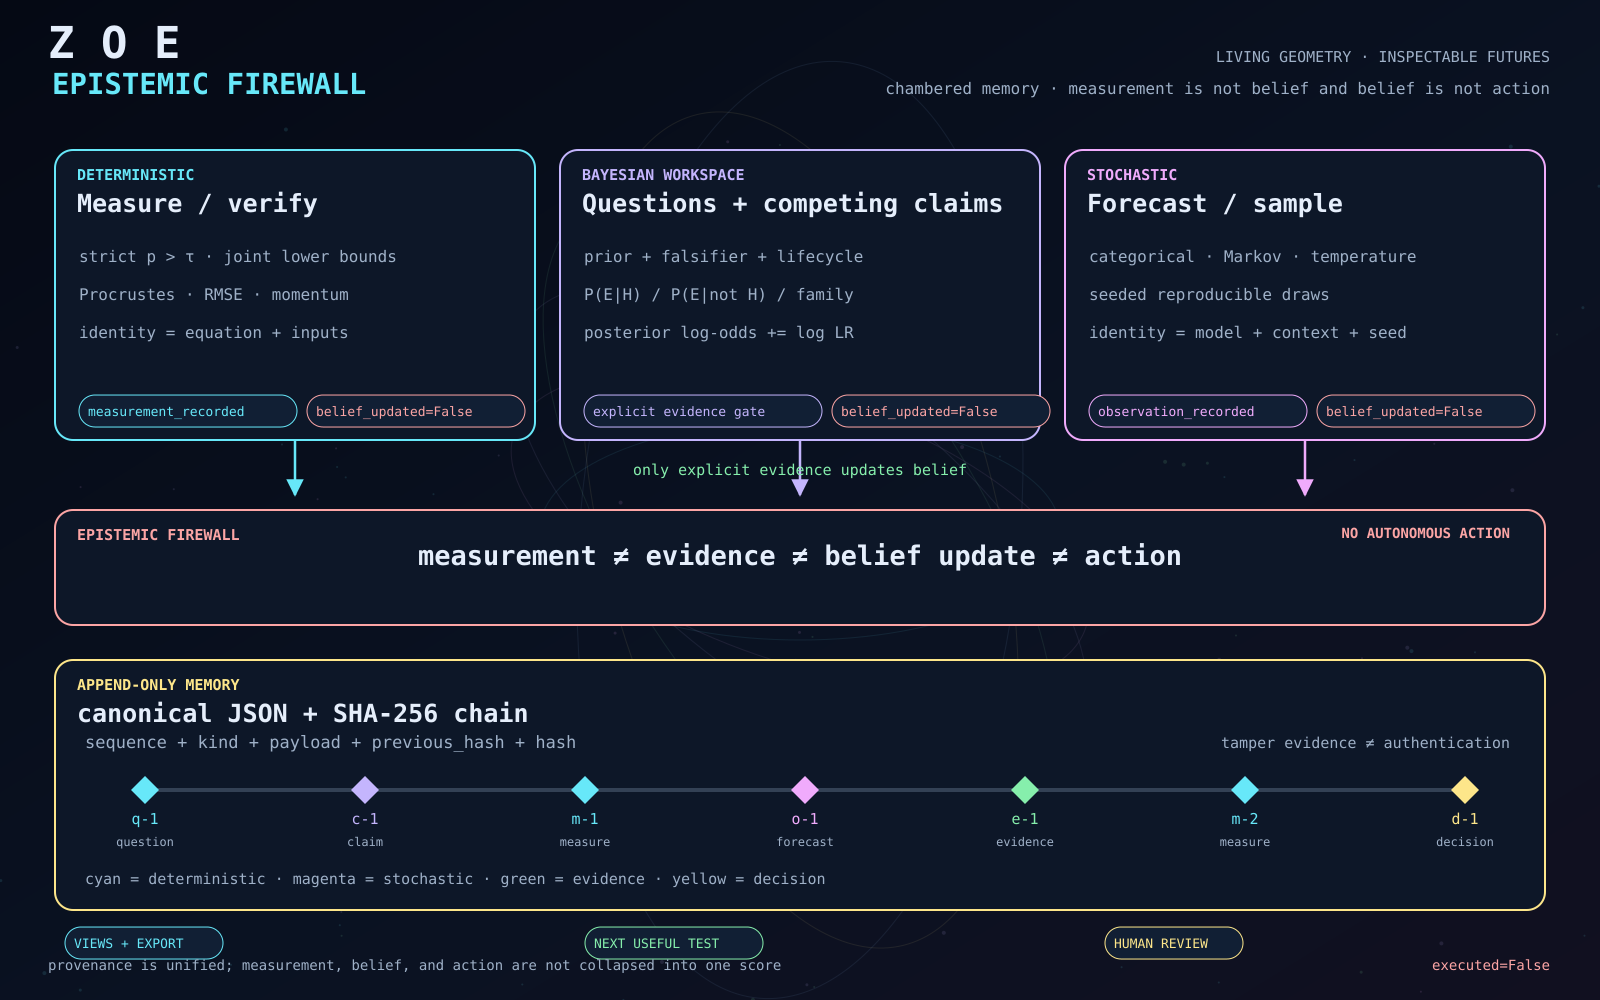
\includegraphics[width=\textwidth]{guiai-lab/docs/images/zoe-visuals/01-epistemic-firewall.png}
\caption{The epistemic firewall separates measurement, evidence, belief updates, and actions while retaining a unified append-only history.}
\end{figure}

The architecture has four cooperating but distinct parts:
\begin{itemize}[nosep]
  \item \textbf{HELEN:} lazy geometry, accessible-volume controls, and compressed held-out predictions.
  \item \textbf{Ablation + GEM:} native GTK, Spatial IR, Lab sessions, VDI replay, and evidence export.
  \item \textbf{Cerotto GEM:} read-only forensic case inspection, guarded native actions, vault timelines, accessible-volume charts, and an optional user-selected agent terminal.
  \item \textbf{BRAIN and the field notebook:} observation state, deterministic recommendations, Bayesian evidence, chamber memory, and next-test selection.
\end{itemize}

PALA is an optional recovery companion. It supplies signature carving, deleted-inode recovery, NTFS cluster-run reconstruction, FAT32 recovery, container expansion, and hash-rich JSON reports. Zoe does not require PALA to run, and PALA does not make recovered content authentic, safe, or complete.

\section{Accessible volume and forecast measurement}
Let $\mathcal O$ be a finite vocabulary and $P(a\mid h_T(S))$ the probability of alternative $a$ after context $S$. Accessible volume is
\begin{equation}
A_\tau(S)=\sum_{a\in\mathcal O}\mathbf 1[P(a\mid h_T(S))>\tau].
\label{eq:av}
\end{equation}
The comparison is strict: alternatives exactly at $\tau$ are excluded. The complement and normalized forms are
\begin{equation}
A^c_\tau(S)=|\mathcal O|-A_\tau(S),\qquad
A_{\mathrm{norm},\tau}(S)=\frac{A_\tau(S)}{|\mathcal O|}.
\end{equation}
If four alternatives have probabilities $0.70,0.20,0.08,0.02$, then $A_{0.05}=3$ and $A^c_{0.05}=1$. The count describes breadth, not whether the selected answer is right.

The adaptive comparison uses
\begin{equation}
A_{\alpha,\beta}(x)=\sum_i\mathbf 1[p_i>\max(\beta,\alpha p_{\max}(x))].
\end{equation}
It remains available for ablation because the selected adaptive rule transferred worse than the fixed $\tau=0.05$ rule in the held-out BioBERT experiment.

Forecast measurements can include entropy, maximum probability, top-ten mass, negative log probability, and Brier score. These measurements describe different properties of a distribution and must not be collapsed into one score.

\subsection{Multi-horizon continuations}
For a learned autoregressive model, a candidate continuation has joint probability
\begin{equation}
P_h(a_{1:h}\mid C_t)=\prod_{j=1}^{h}p(a_j\mid C_{t+j-1},a_{<j}).
\end{equation}
Multi-horizon accessible volume counts complete continuations above a threshold:
\begin{equation}
A^{(h)}_\tau(C_t)=\sum_{a_{1:h}\in O^h}\mathbf 1[P_h(a_{1:h}\mid C_t)>\tau],
\qquad
A^{c,(h)}_\tau(C_t)=|O|^h-A^{(h)}_\tau(C_t).
\end{equation}
Exact enumeration costs $|O|^h$ candidates. A restricted candidate set supplies only a lower bound, with included and excluded probability mass reported explicitly. It is not an exact total.

Accessible Momentum is
\begin{equation}
M_{\tau,i}=A_{\tau,i}-A_{\tau,i-1}.
\end{equation}
Zero momentum means equal counts, not identical probabilities or accessible-set membership. Temperature transforms use
\begin{equation}
p'_k(T)=\frac{p_k^{1/T}}{\sum_j p_j^{1/T}},
\end{equation}
which reshapes a distribution but does not retrain a model or establish creativity.

\section{Accessible Q-Volume: annotating causal repertoires}
The preceding measurement can be generalized without changing its strict comparison. For a probability distribution $p$ on a finite labeled space $Z$, define
\begin{equation}
\mathcal A_\tau[p;Z]=\sum_{z\in Z}\mathbf 1[p(z)>\tau],\qquad
\mathcal B_\tau[p;Z]=\{z\in Z:p(z)>\tau\},\qquad \mathcal A_\tau=|\mathcal B_\tau|.
\end{equation}
The original next-token measurement is $A_\tau(S)=\mathcal A_\tau[P_S;\mathcal O]$. Multi-horizon volume changes the space to $Z=\mathcal O^h$. Accessible Q-Volume instead uses possible prior system states $Z=\mathcal X_0$, where $|\mathcal X_0|=N=2^n$ for $n$ binary elements.

For submechanism $m$, current state $x_1$, and transition kernel $K_m$, the causal repertoire is
\begin{equation}
\rho_m(x_0\mid x_1)=\frac{K_m(x_1\mid x_0)\mu(x_0)}{\sum_{x_0'}K_m(x_1\mid x_0')\mu(x_0')},
\end{equation}
with maximum-entropy intervention distribution $\mu$ and the 2009 IIT paper's extrinsic-noise semantics for disengaged connections. A zero normalizer leaves the repertoire undefined. Then
\begin{equation}
QA_\tau(m;x_1)=\sum_{x_0\in\mathcal X_0}\mathbf 1[\rho_m(x_0\mid x_1)>\tau],\qquad
QB_\tau(m;x_1)=\{x_0:\rho_m(x_0\mid x_1)>\tau\}.
\end{equation}
The symmetry is between above-threshold causal pasts and above-threshold output futures. It is not an equivalence between causal reconstruction and forecasting.

\subsection{Threshold filtrations and annotated q-arrows}
For every repertoire, retain the complete labeled family
\begin{equation}
\mathfrak B(m;x_1)=\left(QB_\tau(m;x_1)\right)_{0\leq\tau<1}.
\end{equation}
Since $\tau_1<\tau_2$ implies $QB_{\tau_2}\subseteq QB_{\tau_1}$, this is a filtration. With $\sup\varnothing=0$,
\begin{equation}
\rho_m(x_0\mid x_1)=\sup\{\tau:x_0\in QB_\tau(m;x_1)\}.
\end{equation}
The complete labeled sweep is therefore a lossless level-set representation of a Q-space point. A scalar count sweep without set membership recovers probabilities only up to permutation of state labels. A finite grid is a stepwise approximation, not guaranteed exact recovery. The saved coarse demonstration reports $0.3$, not $1/3$, when reconstructing from its sampled levels.

When adding mechanism $r$ in context $m$, keep the original information measurement:
\begin{equation}
ei(m,r)=D_{\mathrm{KL}}(\rho_{m\cup r}\|\rho_m).
\end{equation}
Annotate it with volume change and the states entering and leaving:
\begin{align}
\Delta QA_\tau(m,r)&=QA_\tau(m\cup r)-QA_\tau(m),\\
B_\tau^{\mathrm{in}}&=QB_\tau(m\cup r)\setminus QB_\tau(m),\\
B_\tau^{\mathrm{out}}&=QB_\tau(m)\setminus QB_\tau(m\cup r).
\end{align}
Thus the annotated arrow retains $(ei,\Delta QA_\tau,B_\tau^{\mathrm{in}},B_\tau^{\mathrm{out}})$ at each declared threshold. Zero volume change does not imply unchanged accessible-set membership. The operator annotates the geometry; it does not replace $\Phi$ or $\gamma$.

\subsection{The checked silent-AND demonstration}
For $\mu=(1/4,1/4,1/4,1/4)$ on states $00,01,10,11$, the silent AND gate rules out only $11$, so $\rho_T=(1/3,1/3,1/3,0)$. Its effective information is
\begin{equation}
EI=D_{\mathrm{KL}}(\rho_T\|\mu)=\log_2(4/3)=0.4150374993\ldots\ \text{bits}.
\end{equation}
At $\tau=0.20$, the before/after volumes are $4$ and $3$, so $\Delta QA=-1$ and $11$ exits. At $\tau=0.30$, they are $0$ and $3$, so $\Delta QA=+3$ and $00,01,10$ enter. The same positive information accompanies opposite volume changes. Accessible Q-Volume is not $\Phi$, and zero volume change does not establish zero integration.

The complete mechanism's sampled sets are $\{00,01,10\}$ at thresholds $0,0.20,0.30$, and the empty set at $\tau=1/3$. Strict inequality excludes equality. The continuous supremum recovers $1/3$ for the first three states and zero for $11$. The native tests check the coarse approximation and a fine-grid maximum error below $0.0001$ for these states.

If an explicitly supplied mapping $C_t=\iota(x_1)$ connects an internal state to a forecast context, the two-way record is
\begin{equation}
\mathfrak V_{\tau,h}(x_1)=\left(QA_{\tau,T}^{\mathrm{past}}(x_1),A_{\tau,h}^{\mathrm{future}}(\iota(x_1))\right).
\end{equation}
The toy has three accessible causal pasts at $\tau=0.20$ and three accessible next-token alternatives at $\tau=0.05$. The forecast is independently supplied; Zoe does not infer $\iota$ or a causal model from a softmax distribution.

\begin{figure}[htbp]
\centering
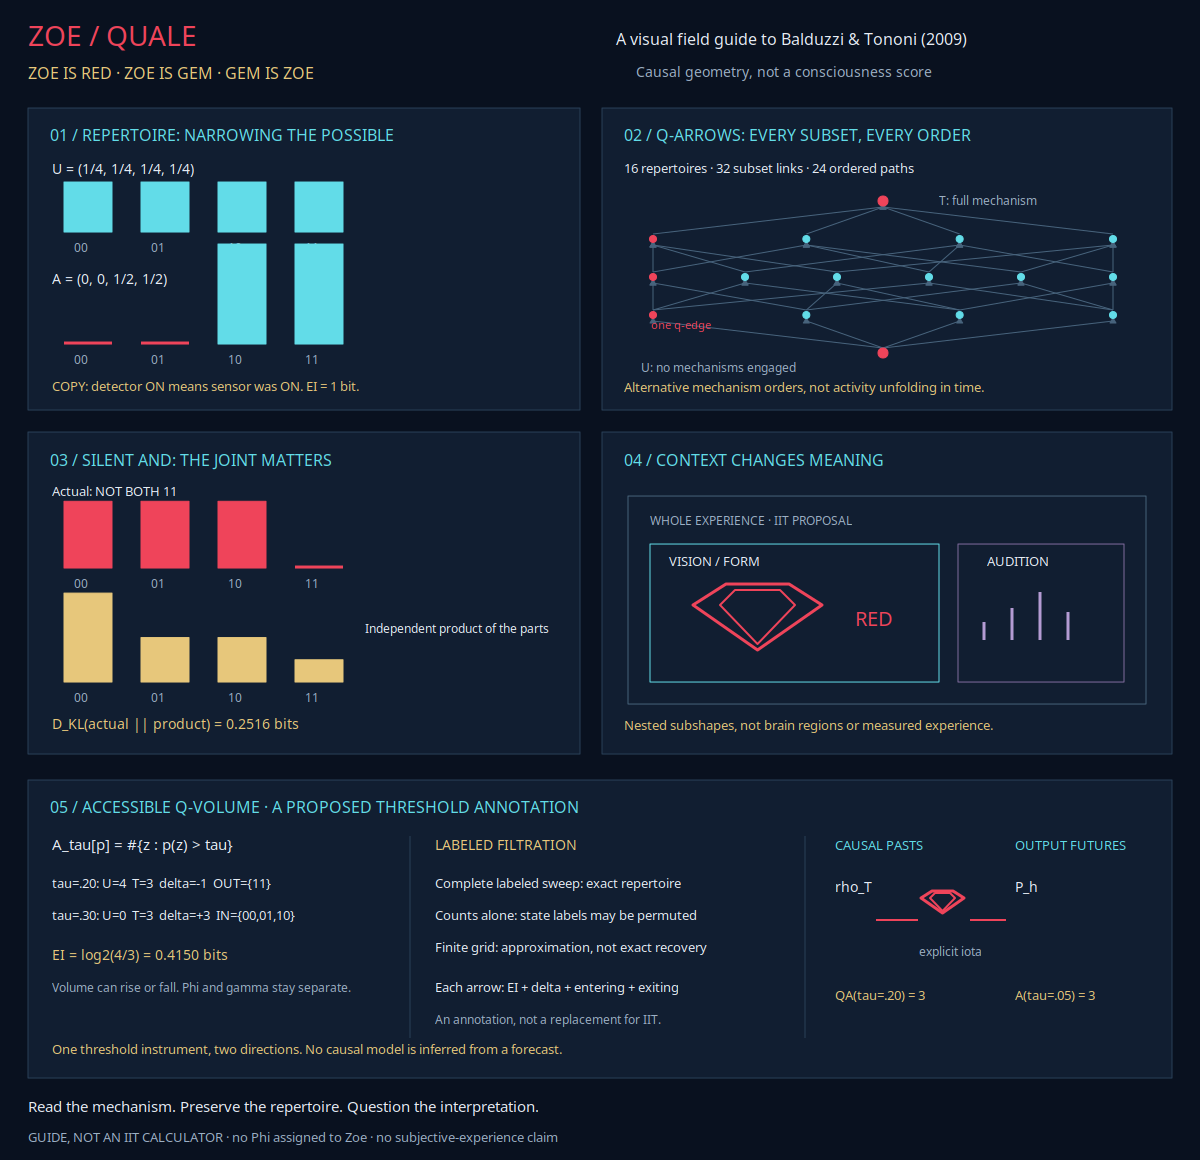
\includegraphics[width=\textwidth,height=0.72\textheight,keepaspectratio]{guiai-lab/docs/images/zoe-qualia.png}
\caption{The Qualia module combines conceptual IIT diagrams with the proposed Accessible Q-Volume annotation and the checked two-way toy. It is not a general IIT calculator or a consciousness measurement.}
\end{figure}

This extension is a proposed construction developed in the present collaboration. It does not reassign credit for the original equation. Its toy arithmetic is verified, but it is not an empirically validated IIT implementation or a claim of global priority. Next-token distributions alone cannot supply Q-repertoires. Normalized and adaptive thresholds may be transferred formally, but their BioBERT results do not validate that new use. Procrustes alignment and HOP remain outside the construction without a calibrated probability distribution.

\section{Temporal and geometric formulations}
Normalized rhythmic intervals use $r_i=(t_{i+1}-t_i)/B$, where $B$ is seconds per beat. Timing error and root-mean-square error are
\begin{equation}
e_i=t_i-\hat t_i,\qquad E=\sqrt{\frac1n\sum_{i=1}^{n}(t_i-\hat t_i)^2}.
\end{equation}
For corresponding one-dimensional onset vectors, Procrustes alignment fits $q_i\approx ap_i+b$ with $a>0$, then reports
\begin{equation}
D(p,q)=\sqrt{\frac1n\sum_{i=1}^{n}\left(q_i-(ap_i+b)\right)^2}.
\end{equation}
This is geometric distance after tempo and translation alignment, not forecast breadth. At least three onsets are needed for a meaningful structural comparison. Temporal reflection is $p'_i=L-p_{n+1-i}$.

The implemented two-dimensional Procrustes modes are similarity, rigid, and affine. Similarity estimates scale, rotation, and translation; rigid fixes scale to one; affine requires at least three noncollinear pairs. Exact landmark alignment does not imply whole-shape, anatomical, or semantic correctness.

\section{Bayesian field notebook}
Questions contain independent binary claims with priors, current posteriors, falsifiers, and lifecycle states. Claims are not forced into a mutually exclusive set. For prior $p$, likelihoods $L_T=P(E\mid H)$ and $L_F=P(E\mid\neg H)$, the update is
\begin{equation}
\operatorname{logit}(p')=\operatorname{logit}(p)+\log\frac{L_T}{L_F},
\qquad \operatorname{logit}(p)=\log\frac{p}{1-p}.
\end{equation}
Every update preserves a belief diff: previous posterior, new posterior, likelihood ratio, log likelihood ratio, prior and posterior log-odds, and evidence source. Evidence may support, challenge, mix, or leave a claim unknown. Negative results are retained.

Evidence families prevent repeated updates from derivative or correlated sources by default. A repeated family requires explicit dependence acknowledgment and adjusted likelihoods. Posteriors remain conditional on the supplied model, not objective truth scores.

Next-test prioritization is a heuristic:
\begin{equation}
\operatorname{priority}=\frac{\text{decision value}\times\text{expected information gain}}{\text{estimated effort}}.
\end{equation}
It ranks inspection only. It is not a probability, reward, or authorization rule. Decisions retain a choice and rationale with \texttt{review\_required=True} and \texttt{executed=False}.

\section{Chambers and unified memory}
The equation registry contains 13 replaceable sections: binary Bayesian updates, strict volume, forecast measurement, adaptive volume, joint volume, momentum, temperature, categorical sampling, Markov steps, bounded continuations, timing RMSE, Procrustes alignment, and inspection priority. Custom functions are registered through the Python API without \texttt{eval}.

Deterministic chambers record reproducible measurements. Stochastic chambers record forecasts, transitions, transforms, and seeded samples. A sampled outcome does not prove correctness. Rejected methods remain available for comparison; quarantined chambers remain inspectable but cannot run.

Events have sequence, kind, payload, previous hash, and hash. The chain uses canonical JSON:
\begin{equation}
h_i=\operatorname{SHA256}\!\left(\operatorname{canonical}(s_i,k_i,p_i,h_{i-1})\right).
\end{equation}
Loading recomputes the complete chain and detects edited or reordered events. Small probability vectors are stored completely. Longer vectors are represented by length and SHA-256 digest to bound memory size. The result is tamper evidence, not cryptographic authentication.

\begin{figure}[htbp]
\centering
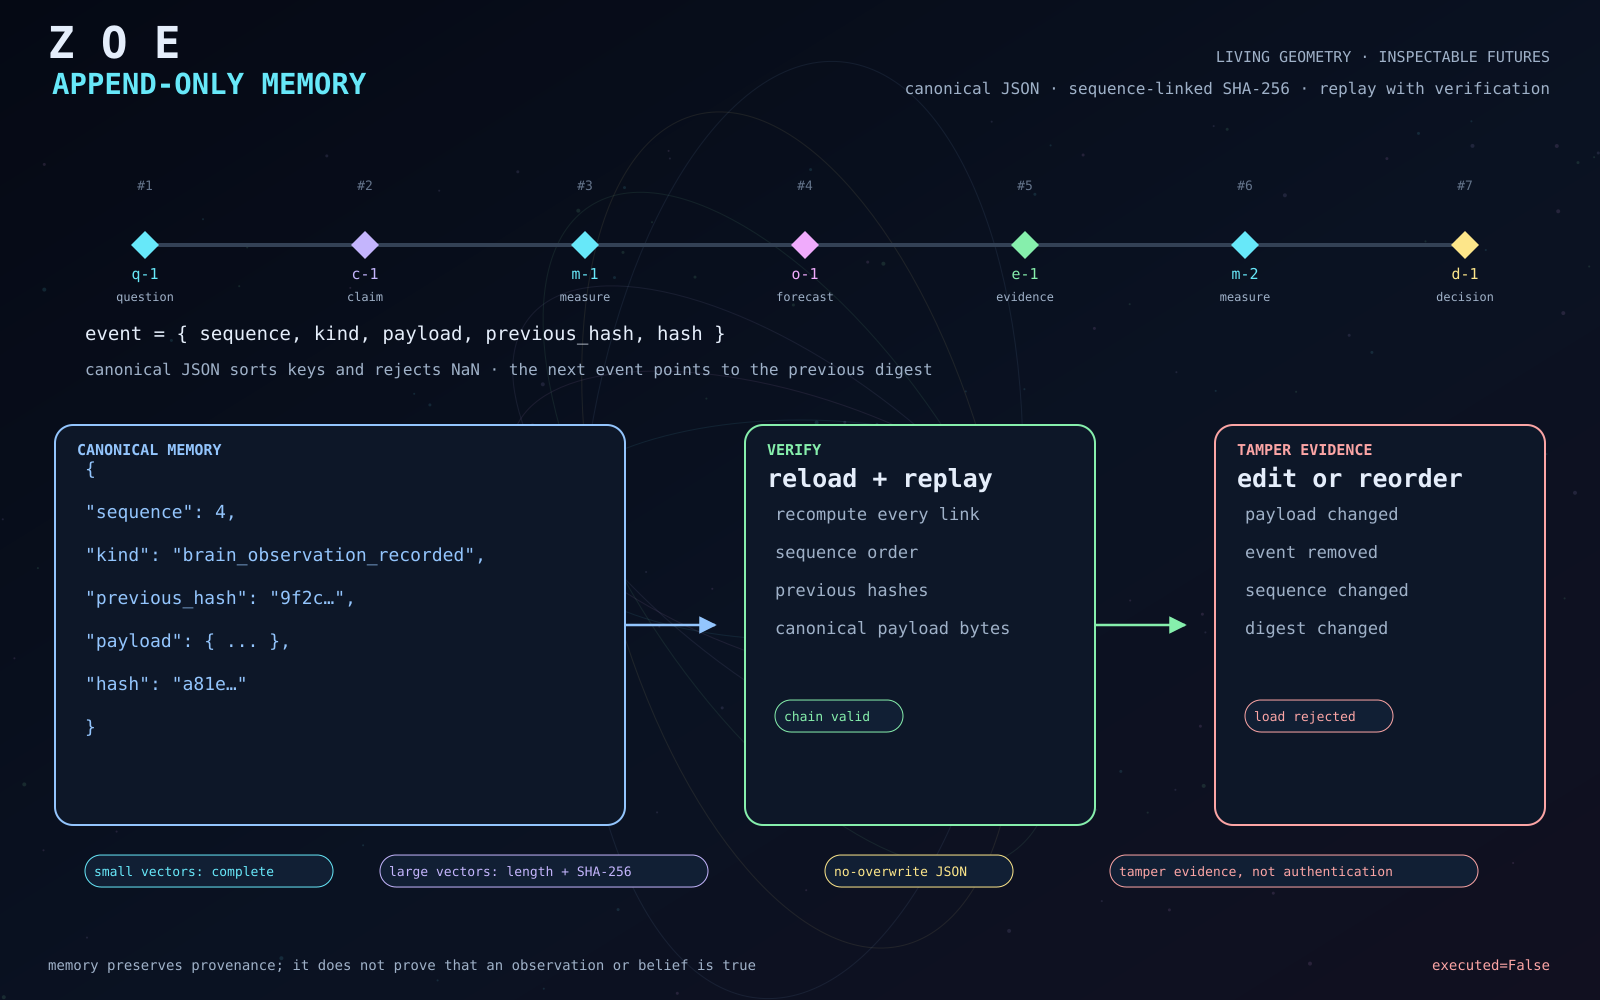
\includegraphics[width=\textwidth]{guiai-lab/docs/images/zoe-visuals/04-memory-chain.png}
\caption{Append-only memory records distinct event kinds and makes alteration visible without claiming identity or authentication.}
\end{figure}

\section{How the GEM versions formed}
\begin{table}[htbp]
\centering
\caption{Native components and their roles in Zoe.}
\small
\begin{tabular}{p{3.1cm}p{5.5cm}p{5.6cm}}
\toprule
Component & What it contributes & What it does not establish \\
\midrule
Ablation GEM & Spatial IR, native GTK, VDI replay, source constraints, Lab evidence & It is not a general proof of semantic correctness. \\
Cerotto GEM & Read-only forensic cases, guard and vault events, charts, guarded native actions & Zoe does not absorb Cerotto's C core, database, vault, or permissions. \\
HELEN & Fast lazy scenes, direct interaction, stored seed-7 predictions & Synthetic forecasts are not real performances or human surprise. \\
Zoe / BRAIN & Observation, recommendation, field memory, native notebooks & Recommendations are not autonomous actions or consciousness. \\
brain-gem & Standalone Bayesian notebook and chambered memory & It is not a new statistical theory or a learned calibration method. \\
PALA & Signature carving, deleted-inode recovery, FAT32, NTFS runs, safe JSON reports & Recovered content is not proof of authenticity, safety, or completeness. \\
\bottomrule
\end{tabular}
\end{table}

The native interface preserves compatibility commands: \texttt{gem zoe}, \texttt{gem master}, \texttt{gem brain}, \texttt{gem atlas}, and standalone \texttt{gem-helen}. The standalone \texttt{brain-gem} package exposes \texttt{brain-gem field} and \texttt{brain-gem notebook}. This separation lets HELEN remain lightweight while Zoe carries the integrated environment.

\section{Experimental evidence}
\subsection{Original accessible-volume studies}
The original Ablation + GEM measurement produced concentrated next-token distributions, repeated bit-identical input IDs and probabilities, and controlled context perturbations. XLNet-Base and XLNet-Large query streams extended the measurement to held-out targets with leakage checks. Sixteen additional model comparisons independently verified every threshold count, target rank, entropy, top-ten mass, top-token ordering, and raw-array hash.

The BioBERT study used 120 cases from 30 documents with document-grouped splits. The original $\tau=0.05$ rule achieved AUROC $0.7737$ and AUPRC $0.7978$, compared with adaptive values $0.7008$ and $0.6599$. The adaptive rule improved validation measurements but transferred worse to unseen documents. This is a direct warning against treating a more complicated threshold as inherently better.

\subsection{HOP is a rejected baseline}
The Harmonic Osculating Predictor used composed rotations to extrapolate hidden-state trajectories. On 1,647 positions it achieved 11.3\% top-1 and 21.4\% top-5 accuracy, compared with 41.3\% and 60.0\% for linear velocity and 46.6\% and 66.6\% for the model. HOP therefore remains a rejected deterministic baseline. It supplies no categorical accessible volume.

The experiment also rejected unsupported interpretations: non-accumulating rotations do not imply an arc, arbitrary hidden states need not be collinear, curvature alone does not imply exponential error growth, and musical metaphors do not establish transformer dynamics.

\subsection{Synthetic and real rhythm experiments}
The synthetic experiment used eight motifs, 60 training and 20 held-out variations per motif, randomized tempo, and jitter. Forward top-1 was 84.375\% (1,620/1,920), retrograde 58.958\% (1,132/1,920). Log-loss was 0.338856 versus 2.898662, while sweep areas were 0.647474 and 0.649180. The retrograde predictor was often confidently wrong: forecast breadth stayed nearly unchanged as correctness fell.

The Magenta Groove experiment used 514 usable 4/4 performances, 396 training and 118 test performances with disjoint recording sessions, 218,033 training windows, and 121,392 predictions per condition. Forward, reversal-transfer, and backward-matched top-1 values were 17.33\%, 16.01\%, and 17.06\%; mean accessible volumes over the sweep were 1.886, 1.885, and 1.886. Backward-matched log-loss was 3.183, slightly lower than forward 3.194. Reversed rhythms were learnable, while direct reversal transfer was worse.

Nightingale supplied 420 files with 139,839 training positions and 57,113 predictions per direction. Classical achieved 68.3\%/67.9\% forward/retrograde top-1, jazz 49.5\%/47.1\%, and folk 61.9\%/61.4\%. Jazz was least predictable and had the broadest forecasts. Reversal effects were small. The saved Nightingale evidence is aggregate-only and does not supply individual per-onset distributions.

\subsection{Bayesian field example}
The DEMOMENU notebook asks what DEMOMENU is in the 1986 \emph{Programmer's Guide to GEM}. It retains the primary DEMO.H definition, the counterevidence of version-dependent appearance, initialization code, a strict measurement, a seeded stochastic chamber, and a next-test recommendation. Its value is not the percentage alone: the complete belief history is inspectable.

\begin{figure}[htbp]
\centering
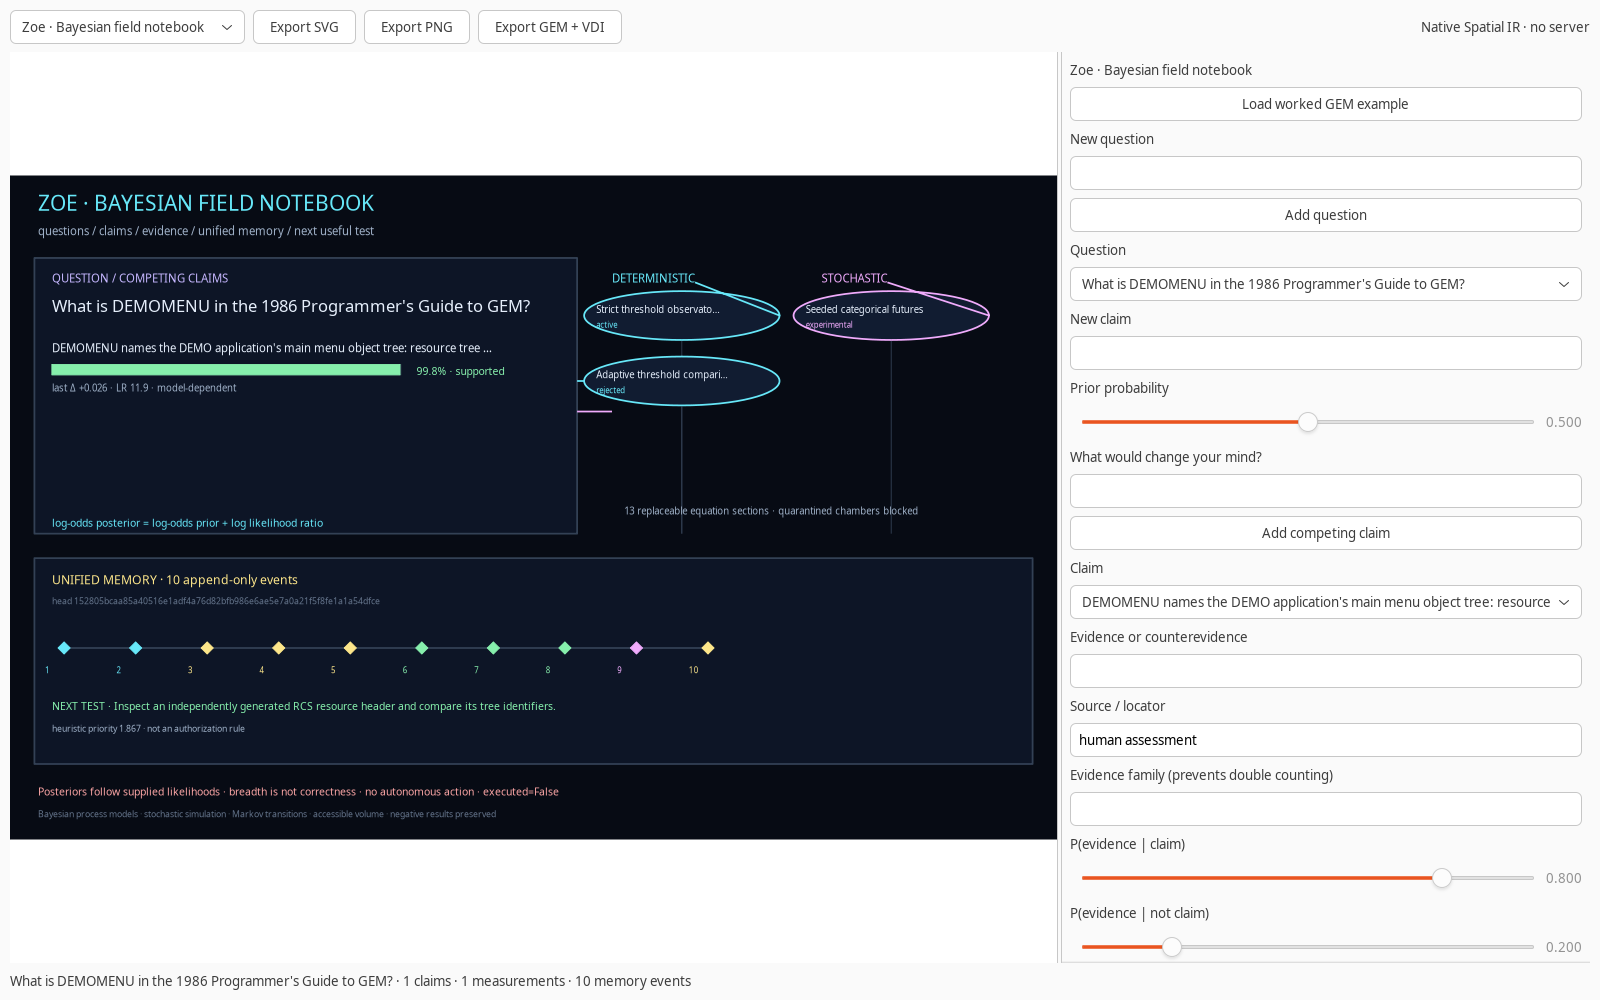
\includegraphics[width=\textwidth]{guiai-lab/docs/images/zoe-field-notebook.png}
\caption{The native Bayesian field notebook: posterior state, chamber states, append-only memory, and next useful test.}
\end{figure}

\section{Verification and reproducibility}
\begin{table}[htbp]
\centering
\caption{Current verification matrix.}
\small
\begin{tabular}{p{4.2cm}p{3cm}p{7cm}}
\toprule
Area & Result & Scope \\
\midrule
Zoe native & 25 passed & X11 observation, notebook, host launch, Allen atlas, research, and export workflows. \\
Zoe headless & 21 passed, 4 native-only skips & 25 tests total: core, Allen atlas, memory, CLI, and evidence behavior without a display. \\
brain-gem headless & 13 passed, 3 native-only skips & 16 tests total: standalone notebook, chambers, memory, and CLI behavior. \\
Broader GEM native & 20 passed & Original GEM constraints, VDI, replay, native dragging, and module exports. \\
Accessible Q-Volume & Toy arithmetic passed & $-1$ and $+3$ volume changes, $EI=0.4150374993$ bits, strict equality, labeled sweeps, finite approximation, and two-way JSON. \\
Research conformance & 17 passed & Strict volume, Procrustes, toy continuations, Groove, Nightingale, and Bayesian updates. \\
Original model cases & 16 verified & Saved distributions, ranks, threshold counts, entropy, and hashes. \\
BioBERT & 120 cases, 54 candidates & Independent AUROC/AUPRC and split recomputation. \\
Cerotto & 64 normal, 64 sanitizer passed & One EWF-dependent skip per suite; real GTK, guard, vault, and integration behavior. \\
PALA & 25 Rust tests, 125 integration checks & Recovery, format, lint, release, and integration behavior; two optional skips. \\
Interactive browser & 23 particles, zero external requests/errors & Desktop, mobile, reduced motion, field details, and controls. \\
Packaging & Wheel and source distributions passed & Installed notebook, HELEN asset, conformance, and export checks. \\
\bottomrule
\end{tabular}
\end{table}

The broader GUIAI stress suite also contains unrelated investigation-CLI and saved-layout failures. Those failures are not used as evidence for Zoe's focused integration results. Cerotto-specific bridge execution was not separately revalidated as part of Zoe.

\section{Applications and boundaries}
Zoe can help people inspect alternatives rather than only final answers. Artists can use geometry, orbital fields, stochastic textures, and exportable scenes. Researchers can preserve competing explanations, negative results, and the evidence for the next experiment. Forensic users can connect guarded actions to evidence rather than treating a forecast as permission.

Potential future applications include biological and genetic research notebooks, timing studies, and brain-mapping workflows. Zoe could help structure hypotheses, evidence families, and uncertainty. These are possibilities for new experiments, not demonstrated clinical, biological, neurological, or diagnostic capabilities. Zoe does not currently map the human brain, diagnose disease, model consciousness, or guarantee beneficial actions.

The strongest lesson is not that a single equation predicts everything. It is that a system can make uncertainty inspectable without turning it into false certainty. Forecast breadth, correctness, belief, and action remain separate.

\section{Reproduction}
From the Zoe checkout:
\begin{lstlisting}
export MASTER_GEM_RESEARCH_ROOT=/path/to/next-token-predictability
PYTHONPATH=guiai-lab python -m guiai.gem zoe
PYTHONPATH=guiai-lab python -m guiai.gem zoe --module field
PYTHONPATH=guiai-lab python -m guiai.gem notebook --output zoe-field.json
PYTHONPATH=guiai-lab python -m guiai.gem notebook zoe-field.json --output zoe-field.svg
\end{lstlisting}
For standalone BRAIN GEM:
\begin{lstlisting}
python -m pip install /path/to/brain-gem
brain-gem field
brain-gem notebook --output field-memory.json
brain-gem notebook field-memory.json --output field-memory.svg
\end{lstlisting}
The research root supplies the saved Groove NPZ and Nightingale reports. The 98 MB Groove archive is referenced by path and hash rather than embedded in this PDF. The complete demo memory, conformance contract, verification summary, source code, and visual evidence are embedded as attachments.

\section{Conclusion}
Zoe is a working native laboratory for living geometry and inspectable futures. It demonstrates that accessible volume can measure breadth, deterministic and stochastic processes can share an equation registry, Bayesian updates can remain inspectable, and memory can be unified without erasing the distinction between measurement, evidence, belief, and action. Its value is practical: a researcher can see what might happen, measure what happened, understand why a belief changed, and choose what to investigate next without pretending that the system knows more than it does.

\appendix
\section{Evidence identity and attachments}
The saved evidence is identified by these SHA-256 digests:
\begin{lstlisting}
Groove predictions.npz
61e2be13296cd306cf9552840b1f0f51eb9ba02fe6a7777d0f5b216a8d4c51c1
HELEN seed-7 artifact
e94671b50c4063900ee248559677402af602839edc1349bda70eb16514de8da9
\end{lstlisting}
The conformance contract, demo memory, verification summary, and this paper's source are included as attachments. The paper also embeds native screenshots, five mechanism diagrams, source scripts, and the research reports needed to inspect the PoC offline.

\embedfile{paper/zoe.tex}
\embedfile{paper/zoe-for-everyone.tex}
\embedfile{paper/zoe-field-demo.json}
\embedfile{paper/verification-summary.json}
\embedfile{evidence/master-gem/conformance.json}
\embedfile{evidence/rhythm-midi/report.json}
\embedfile{evidence/rhythm-lab/results.json}
\embedfile{evidence/verification/model-comparison-summary.json}
\embedfile{evidence/verification/biobert-optimization.json}
\embedfile{evidence/verification/verify-model-comparison.py}
\embedfile{evidence/verification/verify-biobert-optimization.py}
\embedfile{evidence/rhythm-hop/hop-experiment.py}
\embedfile{evidence/rhythm-hop/rhythm-accessible-volume.py}
\embedfile{guiai-lab/guiai/gem/brain.py}
\embedfile{guiai-lab/guiai/gem/field.py}
\embedfile{guiai-lab/guiai/gem/atlas.py}
\embedfile{guiai-lab/guiai/gem/atlas_view.py}
\embedfile{guiai-lab/guiai/gem/cli.py}
\embedfile{guiai-lab/guiai/gem/research.py}
\embedfile{guiai-lab/guiai/gem/helen_onset.py}
\embedfile{guiai-lab/stress/zoe_stress.py}
\embedfile{guiai-lab/docs/ZOE.md}
\embedfile{guiai-lab/docs/QUALIA.md}
\embedfile{guiai-lab/guiai/gem/qualia.py}
\embedfile{guiai-lab/docs/images/zoe-qualia.png}
\embedfile{evidence/qualia/accessible-q-volume.json}
\embedfile{guiai-lab/docs/images/zoe-brain.png}
\embedfile{guiai-lab/docs/images/zoe-field-notebook.png}
\embedfile{guiai-lab/docs/images/zoe-research.png}
\embedfile{guiai-lab/docs/images/cerotto-gem.png}
\embedfile{guiai-lab/docs/images/zoe-visuals/01-epistemic-firewall.png}
\embedfile{guiai-lab/docs/images/zoe-visuals/02-belief-diff.png}
\embedfile{guiai-lab/docs/images/zoe-visuals/03-chambers.png}
\embedfile{guiai-lab/docs/images/zoe-visuals/04-memory-chain.png}
\embedfile{guiai-lab/docs/images/zoe-visuals/05-next-test.png}
\embedfile{assets/master-gem-interactive.html}

\begin{thebibliography}{9}
\bibitem{kloster2026significance}
Nicholas Michael Kloster. \emph{The Significance of Accessible Volume}. November 2026. Original equation created March 6, 2026. \url{https://github.com/Ablation-Tool/next-token-predictability}.
\bibitem{ablation}
Ablation-Tool. \emph{Ablation and GUIAI Lab}. \url{https://github.com/Ablation-Tool/ablation}.
\bibitem{gemhelen}
Ablation-Tool. \emph{GEM HELEN}. \url{https://github.com/Ablation-Tool/gem-helen}.
\bibitem{cerotto}
Ablation-Tool. \emph{CEROTTO: native forensic workbench and guarded evidence actions}. \url{https://github.com/Ablation-Tool/cerotto}.
\bibitem{pala}
Ablation-Tool. \emph{PALA: file and data recovery}. \url{https://github.com/Ablation-Tool/PALA-rust}.
\bibitem{magentagroove}
Magenta. \emph{Groove MIDI Dataset v1.0.0}. CC BY 4.0. \url{https://magenta.tensorflow.org/datasets/groove}.
\bibitem{nightingale}
Nightingale AI. \emph{MIDI Data}. \url{https://github.com/nightingale-ai/midi-data/}.
\bibitem{gemguide}
Balma and Fitler. \emph{Programmer's Guide to GEM}. 1986. VDI primitives, generalized drawing, raster operations, and application patterns.
\bibitem{iit2009}
David Balduzzi and Giulio Tononi. \emph{Qualia: The Geometry of Integrated Information}. PLOS Computational Biology, 2009. \url{https://doi.org/10.1371/journal.pcbi.1000462}.
\bibitem{stability}
Seyed Yadavar Nikravesh. \emph{Nonlinear Systems Stability Analysis}. Equilibrium definitions, Lyapunov's second method, phase-space structure, and time-delayed systems.
\end{thebibliography}

\end{document}
